\documentclass[12pt,letterpaper]{article}
\usepackage[utf8]{inputenc}
\usepackage[T1]{fontenc}
\usepackage{graphicx}
\usepackage{enumitem}
\usepackage{float}
\usepackage{amsmath}
\usepackage{amssymb}
\usepackage{xcolor} 
\usepackage{listings}
\usepackage{hyperref}
%opening
\title{Proyecto de Prolog: Hive}
\author{}
\author{Victor Manuel Cardentey Fundora C411 \and David Guaty Dom\'inguez C412}


\date{}
\lstset{
	columns=fullflexible,
	frame=single,
	breaklines=true,
	postbreak=\mbox{\textcolor{red}{$\hookrightarrow$}\space},
}
\begin{document}

\maketitle
\section*{Estructura del proyecto}
El proyecto consta de 4 m\'odulos:
\begin{enumerate}
	\item app.pl: El m\'odulo encargado de la interacci\'on con el usuario mediante una interfaz gr\'afica realizada en pce.
	\item board.pl: El m\'odulo encargado de modelar la estructura actual de las piezas colocadas. Brinda informaci\'on importante sobre el estado actual del juego.
	\item bugs.pl: EL m\'odulo encargado del manejo de los distintos tipos de insectos. Puede calcular los posibles movimientos de cada insecto.
	\item cpu.pl: El m\'odulo encargado de implementar el jugador no humano.
\end{enumerate}

\section*{board.pl}
\subsection*{Modelado del tablero}
	Aunque el juego no presenta un tablero, el modelado de las posiciones de las piezas sit\'ua las piezas en un grid hexagonal infinito. Para modelar un grid hexagonal se tienen varias opciones, en este proyecto se eligi\'o rotar el eje x del grid de tal forma que cada fila de hex\'agonos est\'a desplaza a la derecha por medio hex\'agono con respecto a la anterior. Por ejemplo, un grid hexagonal de 4x4 se ver\'ia as\'i:
	\begin{figure}[H]
		\centering
		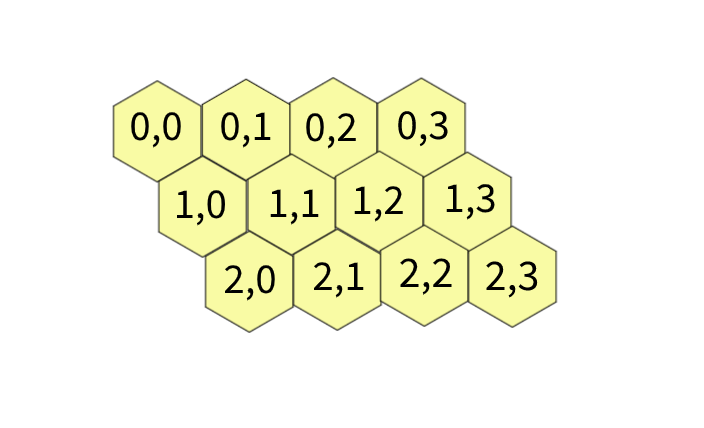
\includegraphics[width=0.7\linewidth]{hexgrid}
		\label{fig:hexgrid}
	\end{figure}

\subsection*{M\'odulo board}
	Teniendo en cuenta la definici\'on de grid hexagonal anterior, se implement\'o el m\'odulo board para obtener informaci\'on acerca del estado actual del juego.
	
	Para saber si dos casillas son adyacentes se tiene el predicado adyacent(X1, Y1, X2, Y2), que triunfa si el hex\'agono con coordenadas X2,Y2 es adyacente al hex\'agono X1, Y1.
	
	Para llevar el estado del juego, board.pl tiene varios predicados din\'amicos que van cambiando de acuerdo a si se coloca una pieza nueva o si se mueve una pieza. 
	
	Para saber si en la celda con coordenadas X,Y existe un insecto en juego se tiene el predicado bug/5.
	
	bug(C,T,X,Y, S) triunfa si existe un bug de color C( con color se hace referencia a un tipo de jugador), de tipo T(hormiga, reina,etc), que est\'a en la posici\'on X,Y. La variable S se refiere a la posici\'on del insecto dentro de la pila de insectos que se puede formar, por ejemplo un escarabajo que est\'e encima de una reina tendr\'a valor S =1, mientras que la reina tendr\'a valor S=0.
	
	A continuaci\'on se explica como se colocan piezas.
	
	\begin{flushleft}
		\textbf{Celdas fronteras}
	\end{flushleft} 
	 Para colocar un insecto en juego, este tiene que ser adyacente a alg\'un insecto de la colmena, si no se cumple esto se romper\'ia la colmena. Por lo que se tiene la definici\'on de \textbf{celda frontera}. Una celda vac\'ia con coordenadas (X,Y) es \textbf{celda frontera} si es adyacente a una celda no vac\'ia.
	 
	 Para saber si una casilla est\'a vac\'ia se tiene: \textit{empty(X,Y):- $\backslash$+ bug(\_,\_, X, Y, \_) }.
	 
	 \paragraph{} 
	 	\begin{flushleft}
	 	\textbf{Manteniendo almacenadas las celdas fronteras y colocando insectos}
	 \end{flushleft} 
	 Para evitar calcular todas las celdas fronteras cada vez que se vaya a colocar un insecto, se tiene el predicado din\'amico frontier/2, frontier(X,Y) triunfa si la celda con posicion (X,Y) es frontera.
	 
	 Para colocar un insecto en juego se tiene el predicado placeBug(C,T,X,Y): coloca el insecto con color C, de tipo T, en la posici\'on X,Y.
	 
	 Al colocar un nuevo insecto en la celda X,Y que es frontera, se expande la frontera de la colmena, almacenando as\'i las nuevas casillas fronteras. En el placebug se tiene la siguiente l\'inea: \textit{ forall(emptyAdyacent(X,Y,X1,Y1), setFrontier(X1,Y1))}. Tambien se setea un nuevo bug, o sea se a\~nade el predicado bug(C,T,X,Y,0) en la base de datos.
	 
	 Nota: El placeBug hace un poco m\'as, porque tambi\'en sirve para el movimiento de las piezas. El placeBug del m\'odulo escoge la altura de la celda con el predicado getCellHeight(X,Y,H) donde se obtiene en H cuantas piezas hay apiladas en la posici\'on X,Y. El insecto con mayor altura dentro de una celda con altura H es H-1. Luego coloca un bug en la altura H seteando bug(C,T,X,Y,H).
	 
	\begin{flushleft}
	 	\textbf{Moviendo insectos}
	 \end{flushleft} 
 	Para saber si un insecto se puede mover se tiene que analizar si la colmena no se divide al remover la pieza del tablero. 
 	
 	\textit{Lema 1: Si un insecto no se puede remover de la colmena, entonces no puede moverse}.
 	
 	Suponga que el insecto a analizar est\'a en la celda A. Se sabe que al removerlo la colmena queda desconexa. Eso significa que existen al menos dos celdas adyacentes a A, X y Y tal que al remover la pieza en A no hay forma de alcanzar a Y partiendo de X. Como dos celdas tienen a lo sumo un par de celdas adyacentes en com\'un se consideraran los siguientes casos:
 	\begin{enumerate}
 		\item A es la \'unica casilla en com\'un con X y Y: En este caso a cualquier lugar al que se mueva el insecto en A quedar\'ian desconexas las celdas X y Y.
 		\item Existe otra celda en com\'un con X y Y: Sea la otra celda en com\'un A1, si el insecto en A logra llegar a A1 entonces puede mantener la colmena conexa, pero note como el insecto no puede ir de A hacia A1, porque incumple la norma de que la ficha tiene que se deslizada, y tampoco puede ir a otra celda intermedia porque dividir\'ia la colmena en su camino. $\blacksquare$

 	\end{enumerate}
 	
 	Luego de que se compruebe que el insecto seleccionado puede moverse, se calculan los posibles destinos a los que puede ir mediante el modulo bugs.pl.
 	
 	Para mover una pieza se utilizan los predicados removeBug y luego placeBug(discutido anteriormente). 
		\begin{flushleft}
		\textbf{Removiendo insectos}
	\end{flushleft} 
	Al remover un insecto se deben actualizar las celdas que dejan de ser fronteras. Las celdas fronteras que dejar\'an de serlo al remover el insecto ser\'an las celdas \textbf{aisladas} que son adyacentes a la celda en la cual est\'a el insecto a remover.
	
	Una celda frontera es aislada si solo posee una celda adyacente no vac\'ia.
	
	\begin{flushleft}
		\textbf{Comprobando si la colmena es conexa}
	\end{flushleft} 
	Para saber si un insecto en la celda X se puede remover se escoge una celda no vac\'ia adyacente a X y se realiza un dfs a partir de ella sin pasar este por la celda X(para esto solo hay que poner en la base de datos que se visit\'o la celda X antes de hacer el dfs). El dfs va insertando en la base de datos un predicado visited(X1,Y1) que triunfa si el dfs ha pasado por esa celda. Al final se comparan la cantidad de celdas visitadas con la cantidad de celdas no vacias, si son iguales entonces el insecto se puede remover y la colmena seguir\'a siendo conexa.
	
	El tablero tambi\'en guarda otras variables que modelan el estado del juego, como por ejemplo la cantidad de piezas que cada jugador posee en la mano, el \'ultimo insecto jugado, entre otras.
	
	\section*{bugs.pl}
	Es el m\'odulo encargado de analizar los posibles destinos de las piezas.
	\begin{flushleft}
		\textbf{Celda Accesible}
	\end{flushleft}
	El concepto de celda accesible es el que permite reconocer las posibles movimientos de la mayor\'ia de las piezas: las piezas que se deslizan.
	
	Se tiene el predicado accessibleCell(X1, Y1, X2, Y2) que triunfa si la celda X2, Y2 es accesible desde la celda X1,Y1 en un movimiento.
	
	Una celda X2,Y2 es accesible desde X1,Y1 si X2,Y2 es una celda frontera adyacente a X1,Y1 y adem\'as X2,Y2 y X1,Y1 comparten una casilla vac\'ia adyacente, esto \'ultimo es para asegurar la condici\'on de que las piezas tengan que deslizarse. Adem\'as se comprueban otros cosas para casos extremos como que la pieza trate de moverse hacia una \textbf{celda aislada}.
	
	Para obtener los destinos de cada pieza se supone que pueden ser removidas, el concepto de celda accesible asegura que la pieza se mueva siempre por la colmena sin dividirla en dos.
	
	\begin{flushleft}
		\textbf{Reina}
	\end{flushleft}
	Para la reina, todos sus posibles destinos son simplemente las celdas accesibles a ella.
	
	\begin{flushleft}
		\textbf{Escarabajo}
	\end{flushleft}
	El escarabajo puede moverse a sus celdas accesibles o cualquiera de las celdas adyacentes a el que no est\'en vac\'ias.
	
	\begin{flushleft}
		\textbf{Saltamontes}
	\end{flushleft}
	Para analizar los posibles destinos del saltamontes, para cada celda adyacente no vac\'ia a \'el, se realiza lo siguiente: Sea la celda del saltamonte X,Y y la celda adyacente no vac\'ia X1, Y1. Se forma el vector V(X1 - X, Y1 -Y) y se avanza en esa direcci\'on hacia X3,Y3. Si X3,Y3 est\'a vac\'ia, X3,Y3 se cuenta como posible destino, si no se repite el proceso hasta encontrar una celda frontera.
	\begin{flushleft}
		\textbf{Araña}
	\end{flushleft}
	Para la araña se programa los posibles destinos por la definici\'on. Dada la posicion X1,Y1 de la ara\~na se encuentran (X2,Y2),(X3,Y3),(X4,Y4), tal que accesible($X_i, Y_i, X_{i+1}, Y_{i + 1}$), i= 1,2,3 y adem\'as todas las celdas sean distintas. 

	\begin{flushleft}
	\textbf{Hormiga}
	\end{flushleft}
	Para la hormiga se hace un dfs que va agregando a la base de datos el predicado din\'amico destination(X,Y) que triunfa si el dfs ha visitado la celda X,Y. El dfs visita una celda si esta es accesible desde la celda actual en la que se est\'a analizando el dfs.
	
	\begin{flushleft}
		\textbf{Mariquita}
	\end{flushleft}
	Al igual que con la ara\~na se procede por definici\'on. Dada la posici\'on de la mariquita X1,Y1 se encuentran (X2,Y2), X3,Y3), (X4,Y4) tal que X2,Y2 sea adyacente no vac\'ia a X1,Y1; X3,Y3 sea adyacente no vac\'ia a  X2,Y2 y X4,Y4 sea adyacente vac\'ia a X3,Y3.
	
	\section*{cpu.pl}
	El m\'odulo cpu contiene una implementaci\'on del algoritmo minimax para obtener la pr\'oxima jugada. Mediante varias m\'etricas y pesos asociados a dichas m\'etricas se forma una heur\'istica para evaluar un estado del juego y determinar quien tiene la ventaja. Para optimizar la b\'usqueda se realiz\'o el pruning Alpha-beta, en el cual se mantienen dos valores, uno almacena la m\'inima puntuaci\'on que el jugador que maximiza tiene asegurado(alpha) y otro almacena la mayor puntuaci\'on que el jugador que minmiza tiene asegurada(beta). Si en alg\'un momento beta < alpha el nodo actual que se est\'e analizando no necesita expandirse m\'as, porque el adversario puede forzar una jugada que resulte en un peor desempe\~no que el obtenido hasta ese momento.
\end{document}